\documentclass[11pt,a4paper]{article}

\usepackage{graphicx}
\usepackage{caption}
\usepackage{listings}


\title{Wavelet noise}
\date{January 2022}
\author{Florian Durand \\ Université Gustave Eiffel}


\begin{document}

\maketitle


\section{Abstract}
When rendering a 3D noise, generated with Ken Perlin method, projected on 2D surface such as a screen. Most of the time it leads to aliasing and detail loss on certain scale. In this paper we try to find a solution to avoid those problems, while keeping the efficiency, the simplicity and easy control of the method. It is important for high quality rendering to not have any artifacts visible. In this report, we show that an efficient and controlable solution is the use of wavelets to generate noise. 
\section{Introduction}
Noise function is used to generate synthetic textures with natural randomness. It can be used to generate visual elements or even for procedural textures.
\begin{figure}[h]
	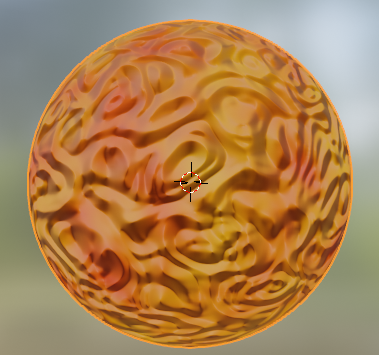
\includegraphics[height=0.25\textwidth]{pictures/texture-noise.png}
	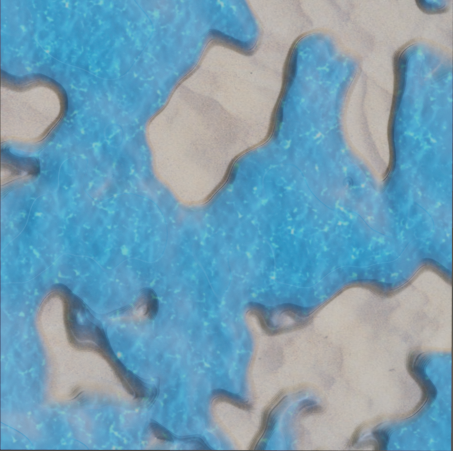
\includegraphics[height=0.25\textwidth]{pictures/landscape.png}
	\centering
	\captionsetup{justification=centering}
	\caption{On the left an example of a procedural noise texture. On the right an example of landscape generated with noise.}
\end{figure}
\\In 2002, Perlin noise was the best noise function used. The benefits of this method was its efficienty, simplicity and easy control. What we understand as easy control, is that we can apply different types of signal to the random generator to control noise shape. Also noise is generated using coordinates, so there exists 1D, 2D, 3D and 4D(time) noise. At Pixar a computer animation film studio, they realized that noise on a certain scale can lead to aliasing and detail loss. Which means that when they rendered a scene with a far background using noise, we can not recognize the texture and it is not smooth or too smooth. Perlin is not enough band limited, this is the reason why we have too much details leading to aliasing. High frequencies not visible are the one that have impact on a certain scale. A good solution found was to use wavelets, to avoid these high frequencies.
\section{Wavelets}

To construct band-limited noise methods based on sinc filters could have been used. Instead they chose to use wavelets because of the wide variety of basis function that can be used. Using wavelets we need to use a refinable function thus when up scaling we keep the same set of functions. However when down scaling we lose some informations as residual. 

\section{Method description}

\begin{enumerate}
\item Create a random noise image $R$
\item Downsample image $R$ to create an half-size image $R_\downarrow$
\item Upsample image $R_\downarrow$ to an new $R$ size image $R_\uparrow$
\item Substract image $R_\uparrow$ from the image $R$ to create image $R_{\uparrow\downarrow}$
\end{enumerate}
When downsampling only representable part are kept, then by upsampling and substracting we remove not representable part of the noise.

\section{Advantages}

\begin{enumerate}
\item This method can be applied to any dimension.
\item This method uses integers parameters. It's not a problem for float values, as it converges fast.
\item Using Gaussian distribution, we can controll the noise distribution.
\end{enumerate}


\section{Conclusion}

Wavelet noise is a well suited solution to avoid detail loss and aliasing when scaling noise for 3D scene rendering. The method is pretty efficient until the repeating patterns are not a problem for the use. However it's particularly focusing on rendering specifities, this method is not generic at all. Most of the functions used are based on the knowledge of how a scene is rendered. Band weight is easy to control, we can easily use different signals to produce an interesting texture. This method only works on static textures, creating abrut transition would make the noise lose some properties like the orthogonality.

\begin{lstlisting}[language=C]
#define ARAD 16
void Downsample (float *from, float *to, int n, int stride ) {
	float *a, aCoeffs[2*ARAD] = {
	0.000334,-0.001528, 0.000410, 0.003545,-0.000938,-0.008233, 0.002172, 		0.019120,
	-0.005040,-0.044412, 0.011655, 0.103311,-0.025936,-0.243780, 0.033979, 	0.655340,
	0.655340, 0.033979,-0.243780,-0.025936, 0.103311, 0.011655,-0.044412,-0.005040,
	0.019120, 0.002172,-0.008233,-0.000938, 0.003546, 0.000410,-0.001528, 	0.000334};
	a = &aCoeffs[ARAD];
	for (int i=0; i<n/2; i++) {
		to[i*stride] = 0;
		for (int k=2*i-ARAD; k<=2*i+ARAD; k++)
			to[i*stride] += a[k-2*i] * from[Mod(k,n)*stride];
	}
}
\end{lstlisting}
This function was not correct in the nested for, the $k<=2*i+ARAD$ lead to an error as $a[k-2*i]$ can access to the $a[32]$ value but aCoeffs size is 32. In order to avoid this error replace $k<=2*i+ARAD \rightarrow k<2*i+ARAD$.
The article lacks of numerics, mainly on the weight distribution values and also tile size used
\section{Bibliography}

\begin{enumerate}
\item https://graphics.pixar.com/library/WaveletNoise/paper.pdf
\end{enumerate}

\section{old}
Noise function is used to generate synthetic textures with natural randomness. It can be used to generate visual elements or even for procedural textures. In 2002, Ken Perlin noise was the best noise function, despite that nowadays the fractal noise and simplex noise have take on Ken Perlin noise, we will study the Ken Perlin problems. The main problems are that 3D noise projected on 2D surface such as screen can lead to aliasing and detail loss.
\\
Perlin band of noise are limited in the range of frequencies. Using interpolation can help improve noise spectrum but it is expensive.
Perlin benefits are speed, simplicity and easily control. Frequencies range is in power-of-2. These frequencies are composed of useful low frequencies visible and high frequencies that can cause aliasing.
At Pixar they tried to find the best solution to avoid loss of detail and aliasing, they used the wavelets to generate noise. But we can see that their solution lose a lot of detail on far distance. They want to keep the band-limited property.
\\\\


Naive solution would be to use $sinc$ filters to get band-limited signal.
The solution used is wavelet because of the wide variety of basis functions used in renderers and wavelet.
\\\\
$M(x) = \sum\limits_{b=b_{min}}^{b_{max}} w_{b}N(2^{b}x)$
\\
with :
\\
$M(x)\rightarrow$  multiresolution noise
\\
$N(x)\rightarrow$ noise band
\\
$b\rightarrow$ band index
\\
$w_{b}\rightarrow$ free variable to control spectral character
\\
\\
rendering process :
\\
$Pixel(i) = \int S(x)K(x-i)dx$
\\
$S(x)\rightarrow$ the scene being render
\\
$K(x-i)\rightarrow$ Kernel filter centered at pixel i with $K(x) \geq 0$ 
\\
\\
It's not possible to prevent aliasing with all the different conditions of rendering. The method will guarantee no aliasing under ideal conditions.
\\
$S(x)\approx M(2^s(x-k))$
\\
$s\rightarrow$ the scale of the scene at pixel $i$
\\
$k\rightarrow$ is the offset at pixel i
\\\\
$Pixel(i) = \int M(2^s(x-k))K(x-i)dx $ 
\\
$ = \int\sum\limits_{b=b_{min}}^{b_{max}} w_{b}N(2^{s+b}(x-k))K(x-i)dx$
\\
$ = \sum\limits_{j=b_{min}+s}^{b_{max}+s} w_{j-s} \int N(2^{j}x-l)K(x-i)dx $
\\
$s+b\rightarrow j$
\\
$2^{s+b}k\rightarrow l$
\\\\
$N(2^{j}x-l)K(x-i)dx = 0 \rightarrow j\geq0 $
\\
This means that N(x) and K(x) are orthogonal.
\\
And so noise function should vanish when aliasing occur.
\\\\
scale correspond to how much the noise will be at the right scale.
\\
scale -1 = no scale\\
scale > -1 = scale up\\
scale < -1 = scale down\\\\
$F(x) = \sum\limits_{i}f_i \phi(x-i)$\\
A refinable function is needed (when up scaling we keep the same set of functions).
We can use coefficients $f_i^\uparrow$ to upscale the function.\\
$F(x) = \sum\limits_{i}f_i^\uparrow \phi(2x-i)$\\
$f_i^\uparrow =\sum\limits_{k}p_{i-2k}f_k $\\
It is not true for downscaling.\\
$G(x) = G^{\downarrow}(x) + D(x)$\\
$D(x)\longrightarrow$ residual \\
$g_i^\downarrow=\sum\limits_{k}a_{k-2i}g_k $\\
$\int D(2^jx-l)\phi(x-i)dx$\\
Thus, if we build our noise bands in the wavelet space $W_0$, then they can be
scaled to any resolution j and be guaranteed to have no effect on
images at any resolution less than j.
\\
We will uniform quadratric B-spline for our kernel because it close to renderer filters, low degree simple to evaluate and efficient, good for procedural shading.\\\\
1. Create random noise from the basis function\\
2. Downsample $R(x)$\\
3. Upsample $R^{\uparrow\downarrow}(x)$\\
4  $R(x) - R^{\uparrow\downarrow}(x)$\\\\
same for multiple dimensions\\
integer to float is not a problem, it converges fast\\
projected noise pas tout compris\\
noise evaluation using weight, see code\\
this noise can controll statisticall distribution base on guassian distribution.\\
use one noise tile, there is also \\



\end{document}